%!TEX root = widefieldscan.tex
\svnidlong
{$HeadURL$}
{$LastChangedDate$}
{$LastChangedRevision$}
{$LastChangedBy$}

\begin{center}
	\fbox{
		\begin{minipage}{.618\textwidth}
		The file of this section is \url{\svnkw{HeadURL}}, was last changed at: \svnfileday.\svnfilemonth.\svnfileyear \space \svnfilehour:\svnfileminute \space (UTC\svnfiletimezone) and is at revision \svnkw{LastChangedRevision}.
		\end{minipage}
	} 
\end{center}

\section{Results}
\label{sec:Results}
\subsection{Image Merging and Reconstruction}
\label{sec:Image Merging and Reconstruction}
Results of the steps mentioned in section~\ref{sec:materials and methods} are shown in figure~\ref{fig:wide field scan results}. Figure~\ref{fig:subscans} shows exemplary projection images from overlapping subscans prior to correction and normalization. Figure~\ref{fig:merge-proj} shows a merged projection image prior to reconstruction and figure~\ref{fig:merge-rec} shows the end-result of such a wide field scan, a reconstructed slice of the whole sample with a FOV of \SI{5.734}{\milli\meter} which is approximately three times the size of what can be achieved with one single scan.

\begin{figure}
	\renewcommand{\imsize}{.16\linewidth}
	\pgfmathsetlength{\imagewidth}{\imsize} % desired display width of image
	\pgfmathsetlength{\imagescale}{\imagewidth/512} % pixel width of image
	\centering
		\subfloat[Uncorrected projection images from subscans s$_1$--s$_3$, each with a size of 1024$\times$1024 pixels at a resolution of \SI{1.4}{\micro\meter\per pixel}, covering a FOV of approximately \SI{0.7}{\milli\meter}. The scans overlap each other by approximately 100 pixels. 4676 projections have been acquired for the subscans s$_1$ and s$_3$, 1169 projections have been acquired for subscan s$_2$, all over a rotation of \SI{180}{\degree}.]{%
			\label{fig:s1}%
			\includegraphics[width=\imsize]{img/merge/R108C10B-s1}%
			\includegraphics[width=\imsize]{img/merge/R108C10B-s2}%
			\begin{tikzpicture}[x=\imagescale,y=-\imagescale]
				% place image (integer coordinates refer to pixel centers):
				\node[anchor=north west,inner sep=0pt,outer sep=0pt] at (0,0)
					{\includegraphics[width=\imagewidth]{img/merge/R108C10B-s3}};
				\draw[|-|,color=white] (256-64,450) -- (512-64,450) node[midway,above] {\SI{700}{\micro\meter}};
			\end{tikzpicture}
			\label{fig:subscans}
			}
		\renewcommand{\imsize}{.48\linewidth}
		\pgfmathsetlength{\imagewidth}{\imsize} % desired displayed width of image
		\pgfmathsetlength{\imagescale}{\imagewidth/1498} % pixel width of image
		\subfloat[Merged and corrected image from the three subscans shown in subfigure~\subref{fig:subscans}. The merged projections have a size of 2994$\times$1024 pixels at a resolution of \SI{1.4}{\micro\meter\per pixel}. The Subscans s$_1$--s$_3$ overlap each other by approximately 150 pixels, thus the width of the merged projection is smaller than three times the width of the subscans. The projections of the subscans above have been merged into 4676 projections images like the one shown here and were then reconstructed into a tomographic dataset using a filtered back-projection reconstruction algorithm.]{%
			\begin{tikzpicture}[x=\imagescale,y=-\imagescale]
				\node[anchor=north west,inner sep=0pt,outer sep=0pt] at (0,0)
					{\includegraphics[width=\imagewidth]{img/merge/R108C10B-merge}};
				\draw[|-|,color=white] (1242-64,450) -- (1498-64,450) node[midway,above] {\SI{700}{\micro\meter}};
			\end{tikzpicture}
			\label{fig:merge-proj}
			}
		\renewcommand{\imsize}{\linewidth}
		\pgfmathsetlength{\imagewidth}{\imsize} % desired displayed width of image
		\pgfmathsetlength{\imagescale}{\imagewidth/1365} % pixel width of image (image has been resized from 2994*1123, so that scalebar is at the same height without calculating too much...)
		\subfloat[Cropped part of one slice of the tomographic dataset reconstructed from the merged projections, where one is shown in subfigure~\subref{fig:merge-proj}. The halo directly around the lung tissue arises from the paraffin where the sample is embedded in. The bright circular shape inscribed in the square arises from the filtered back-projection, the chosen reconstruction method. The size of the cropped image is 2994$\times$1123 pixels. The small inset on the upper left corner shows an overview over the full slice with a size of 2994$\times$2994 pixels.]{%
			\begin{tikzpicture}[x=\imagescale,y=-\imagescale]
				% place image (integer coordinates refer to pixel centers):
				\node[anchor=north west,inner sep=0pt,outer sep=0pt] at (0,0)
					{\includegraphics[width=\imagewidth]{img/merge/R108C10B-merge1016-crop}};
				\newcommand{\size}{.2\imagewidth}
				\node[anchor=north west,inner sep=0pt,outer sep=0pt] at (0,0)
					{\includegraphics[width=\size]{img/merge/R108C10B-merge1016}};
					\draw[white] (\size,0) -- (\size,-\size) -- (0,-\size);
				\draw[|-|,color=white] (1109-64,450) -- (1365-64,450) node[midway,above] {\SI{700}{\micro\meter}};
			\end{tikzpicture}
			\label{fig:merge-rec}
			}
	\caption{Different stages of a wide field scan of a rat lung sample obtained from a Sprague-Dawley rat 10 days after birth, showing the distal-medial edge of the right lower lung lobe. The sample has been scanned at a beam energy of \SI{12.6}{\kilo\electronvolt}.}
	\label{fig:wide field scan results}	
\end{figure}

\subsection{Quality guided protocol selection}
A sequence of 19 protocols with varying quality has been scanned to assess the simulations. The properties of the scan have been chosen according to a MATLAB-plot---as described in section~\ref{seq:Image Acquisition}---which has been generated with \verb+MATLAB\wfs-sim\main.m+ \todo{only necessary if we provide the code\ldots} for a protocol with the diameter of \SI{3.8}{mm} and three overlapping subscans.

We assessed the image differences for the 19 scanned protocols in such a way that the raw data slices have been binarized using an automated thresholding algorithm method, which chooses the threshold to minimize the intraclass variance of the black and white pixels~\cite{Otsu1979}. The binarization of the images suppresses small variations in the gray values which can occur through the reconstruction for the different protocols. A suitable threshold has been automatically chosen by the thresholding algorithm.

The thresholded slices of each protocol have been compared to the gold standard protocol in such a way that the sum of all pixels of the absolute difference image ($Diff_{Protocol_{i}}$) of the relevant protocol with the gold standard protocol has been taken and this difference image has been summed up to yield an error value ($E_{Protocol_{norm_{i}}}$). Equations~\ref{eq:errorcalculation-a}--\ref{eq:errorcalculation-b} show the details of this calculations.

\begin{eqnarray}
    Diff_{Protocol_{i}} &=& |Slice_{A_{i}}-Slice_{Protocol_{i}}| \label{eq:errorcalculation-a}\\
E_{Protocol_{norm_{i}}} &=& \sum_{x}\sum_{y} Diff_{Protocol_{i}} \label{eq:errorcalculation-b}\\
    E_{Protocol_{norm}} &=& \overline{E_{Protocol_{norm_{i}}}} \pm \sigma(E_{Protocol_{norm_{i}}}) \textrm{ for } i=1:5:1024 \label{eq:errorcalculation-c}
\end{eqnarray}

The error value ($E_{Protocol_{norm}}$ has been calculated for 205 regularly spaced slices of the full dataset (1024 slices). The mean ($\overline{E_{Protocol_{norm_{i}}}}$) and standard deviation of the error have been plotted (shown in figure~\ref{fig:NormalizedErrorPlot}) in such a way that the error has been scaled in arbitrary units from 0 to 1.

We see that---as expected---the normalized error grows with decreasing amount of total obtained projections. The simulated scanning quality shown in figure~\ref{fig:2008c-qualityplot} shows the simulated quality to expect from the scan, while figure~\ref{fig:NormalizedErrorPlot} is a plot of the calculated error of the different protocols compared to protocol A\todo{explain more in depth!!!}.

\begin{figure}
	\centering
		%\documentclass{article}
%\usepackage{tikz,pgfplots}
%\usepackage[pdftex,active,tightpage]{preview}
%\begin{document}
%\begin{preview}

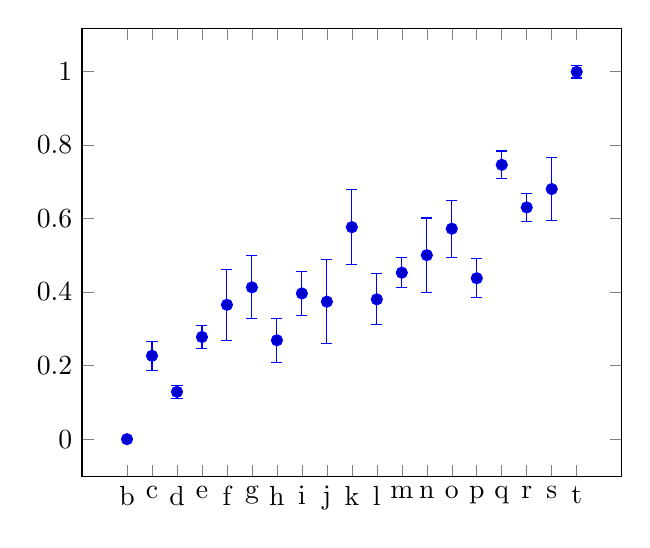
\begin{tikzpicture}
\begin{axis}[%
	%grid=both,%
	%xmajorgrids,%
	xtick={1,2,3,4,5,6,7,8,9,10,11,12,13,14,15,16,17,18,19},%
	xticklabels={b,c,d,e,f,g,h,i,j,k,l,m,n,o,p,q,r,s,t},%
]
% Line plot
\addplot
	plot[ 	%smooth,
	   		only marks,
	      	error bars/.cd,
	      	y dir=both, y explicit %
		]
	coordinates{
	(1,0) 			+- (0,0)
	(2,0.226697)	+- (0,0.0389)
	(3,0.128649)	+- (0,0.0174)
	(4,0.277819)	+- (0,0.0316)
	(5,0.365309) 	+- (0,0.0960)
	(6,0.412726)	+- (0,0.0856)
	(7,0.268849) 	+- (0,0.0598)
	(8,0.396237)	+- (0,0.0589)
	(9,0.373823)	+- (0,0.1148)
	(10,0.576375)	+- (0,0.1020)
	(11,0.380172) 	+- (0,0.0696)
	(12,0.452672)	+- (0,0.0404)
	(13,0.500303)	+- (0,0.1010)
	(14,0.572158)	+- (0,0.0778)
	(15,0.437586)	+- (0,0.0524)
	(16,0.745885)	+- (0,0.0376)
	(17,0.630023)	+- (0,0.0386)
	(18,0.679989)	+- (0,0.0852)
	(19,0.998734)	+- (0,0.0169)
};

\end{axis}
\end{tikzpicture}


% plot erstellt mit MATLAB-File p:\doc\MATLAB\WFS-CompareDMPs\wfs_Compare2008c.m (FromToTo = 1:5:1024)
% und matlab2tikz

%[ 1:19;std(NormCumulativeError);mean(NormCumulativeError)]
%
%ans =
%
%  Columns 1 through 12
%
%    1.0000    2.0000    3.0000    4.0000    5.0000    6.0000    7.0000    8.0000    9.0000   10.0000   11.0000   12.0000
%         0    0.0389    0.0174    0.0316    0.0960    0.0856    0.0598    0.0589    0.1148    0.1020    0.0696    0.0404
%         0    0.2267    0.1286    0.2778    0.3653    0.4127    0.2688    0.3962    0.3738    0.5764    0.3802    0.4527
%
%  Columns 13 through 19
%
%   13.0000   14.0000   15.0000   16.0000   17.0000   18.0000   19.0000
%    0.1010    0.0778    0.0524    0.0376    0.0386    0.0852    0.0169
%    0.5003    0.5722    0.4376    0.7459    0.6300    0.6800    0.9987          	
         	
%
%\end{preview}
%\end{document}
	\caption{Plot of normalized Error for the different protocols. The normalized Error has been calculated in such a way that we have taken the Difference image for Protocol 'x' compared to Protocol 'A' and . The error bars for each protocol show the standard deviation of the error which was calculated for 205 of the 1024 slices for each protocol.}
	\label{fig:NormalizedErrorPlot}
\end{figure}

\subsection{Three dimensional visualizations}
\subsubsection{19 Protocols}
The 19 different protocols which have been obtained from the same sample have been three dimensionally visualized and analyzed using MeVisLab (Version 1.6.1 (2008-09-21 Release), MeVis Medical Solutions AG, Bremen, Germany).
Using a visualization network \todo{exactly explain the network?} we automatically segmented airway segments from the dataset using a region growing algorithm~\cite{wiki:regiongrowing} using the same seed point to extract segments for all protocols.

Two exemplary visualizations of such segment extractions are shown in figure~\ref{fig:BvsT}\todo{explain these extractions in more details}.
\begin{figure}
	\centering
	\renewcommand{\imsize}{.5\linewidth}	
		\subfloat[Overview Protocol B]{%
			\includegraphics[width=\imsize]{img/protocols/BvsT/overviewB}}
		\subfloat[Overview Protocol T]{%
			\includegraphics[width=\imsize]{img/protocols/BvsT/overviewT}}\\
	\renewcommand{\imsize}{.495\linewidth}
		\subfloat[Detailed view of segments of Protocol B]{%
			\includegraphics[width=\imsize]{img/protocols/BvsT/detail-1-B}}\hfill
		\subfloat[Detailed view of segments of Protocol B]{%
			\includegraphics[width=\imsize]{img/protocols/BvsT/detail-1-T}}\\
		\subfloat[Bottom view of underside of Protocol B]{%
			\includegraphics[width=\imsize]{img/protocols/BvsT/detail-2-B}}\hfill
		\subfloat[Bottom view of underside of Protocol T]{%
			\includegraphics[width=\imsize]{img/protocols/BvsT/detail-2-T}}
	\caption{Segmentation of two exemplary protocols, namely B and T.}
	\label{fig:BvsT}
\end{figure}

\subsubsection{some other visualizations}
\renewcommand{\imsize}{.5\linewidth}
\pgfmathsetlength{\imagewidth}{\imsize} % desired displayed width of image
\pgfmathsetlength{\imagescale}{\imagewidth/1293} % pixel width of imagefile used below
\begin{figure}
	\centering
		\subfloat[conventional scan]{
			\label{subfig:overview-s2}%
%			\fbox{%
%				\includegraphics[width=\imsize]{img/widefieldscanning/R108C04C-merge-overview-merge}%
				\begin{tikzpicture}[x=\imagescale,y=-\imagescale]
				\def\x{200}
				\def\y{700}
    				\node[anchor=north west,inner sep=0pt,outer sep=0pt] at (0,0)
	    			{\includegraphics[width=\imagewidth]{img/widefieldscanning/R108C04C-merge-overview-s2}};
%					\draw[|-|,thick] (230,513) -- (724,708) node [midway,below] {\SI{1.4336}{\milli\meter}}; 
%				    %\draw[|-|,thick] (0,0) -- (718,0) node[midway,below] {\SI{1.4336}{\milli\meter}}; 
%				    % 531 px = 1.4336 mm > 100 px = 269.933 um > 1349 px = 500 um
				    \draw[|-|,thick] (\x,\y) -- (185+\x,\y) node [midway,above] {\SI{500}{\micro\meter}}; 
				\end{tikzpicture}%
%			}%
		}%
		\subfloat[wide field scan]{
			\label{subfig:overview-merge}%
%			\fbox{%
%				\includegraphics[width=\imsize]{img/widefieldscanning/R108C04C-merge-overview-merge}%
				\begin{tikzpicture}[x=\imagescale,y=-\imagescale]
				\def\x{200}
				\def\y{650}
    				\node[anchor=north west,inner sep=0pt,outer sep=0pt] at (0,0)
	    			{\includegraphics[width=\imagewidth]{img/widefieldscanning/R108C04C-merge-overview-merge}};
%					\draw[|-|,thick] (11,517) -- (858,754) node [midway,right] {\SI{3.8444}{\milli\meter}}; 
%				    \draw[|-|,thick] (0,0) -- (1011,0) node[midway,below] {\SI{3.8444}{\milli\meter}}; 
				    % 880 px = 3.8444 mm > 100 px = 437 um > 114 px = 500 um
					\draw[|-|,thick] (\x,\y) -- (228+\x,\y) node [midway,above] {\SI{1}{\milli\meter}}; 
				\end{tikzpicture}%
%			}%
		}%
	\caption{Three dimensional visualization of the distal-medial edge of the right lower lung lobe of a Sprague Dawley rat. The grey structure in the background shows a semitransparent view of the sample with segmented airways. The foreground shows isosurfaces of terminal airways that have been extracted using a region growing algorithm (green and red for \subref{subfig:overview-s2}, green and red yellow for \subref{subfig:overview-merge}.}
	\label{fig:overview}
\end{figure}

\pgfmathsetlength{\imagewidth}{\imsize} % desired displayed width of image
\pgfmathsetlength{\imagescale}{\imagewidth/1299} % pixel width of imagefile used below
\begin{figure}
	\centering
		\subfloat[conventional scan]{%
			\label{subfig:down-s2}%
%			\fbox{
%				\includegraphics[width=\imsize]{img/widefieldscanning/R108C04C-merge-down-s2}%
				\begin{tikzpicture}[x=\imagescale,y=-\imagescale]
				\def\x{750}
				\def\y{700}
    				\node[anchor=north west,inner sep=0pt,outer sep=0pt] at (0,0)
    				{\includegraphics[width=\imagewidth]{img/widefieldscanning/R108C04C-merge-down-s2}};
%				\draw[|-|,thick] (350,290) -- (350,595) node [midway,below] {\SI{1.4336}{\milli\meter}}; 
%			   	 \draw[|-|,thick] (0,0) -- (0,640) node[midway,below] {\SI{1.4336}{\milli\meter}};
			   	 % 305 px = 1.4336 mm > 100 px = 470 um > 106 px = 500um
					\draw[|-|,thick] (\x,\y) -- (106+\x,+\y) node [midway,above] {\SI{500}{\micro\meter}}; 
				\end{tikzpicture}%
%			}%
		}%\\%
		\subfloat[wide field scan]{
			\label{subfig:down-merge}%%
%			\fbox{%
%				\includegraphics[width=\imsize]{img/widefieldscanning/R108C04C-merge-down-merge}%
				\begin{tikzpicture}[x=\imagescale,y=-\imagescale]
				\def\x{775}
				\def\y{800}
    				\node[anchor=north west,inner sep=0pt,outer sep=0pt] at (0,0)
    				{\includegraphics[width=\imagewidth]{img/widefieldscanning/R108C04C-merge-down-merge}};
%			    	\draw[|-|,thick] (547,19) -- (498,775) node [midway,right] {\SI{3.8444}{\milli\meter}}; 
%					\draw[|-|,thick] (0,0) -- (0,882) node[midway,right] {\SI{3.8444}{\milli\meter}}; 
				    % 758 px = 3.844 mm > 100 px = 507 um > 99 px = 500um
					\draw[|-|,thick] (\x,\y) -- (198+\x,\y) node [midway,above] {\SI{1}{\milli\meter}}; 
				\end{tikzpicture}%
%			}%
		}%
	\caption{Three dimensional visualization of the distal-medial edge of the right lower lung lobe of a Sprague Dawley rat (same as in figure~\ref{fig:overview}). View from the underside of the sample}
	\label{fig:down}
\end{figure}

%\renewcommand{\imsize}{.618\linewidth}
\renewcommand{\imsize}{\linewidth}
\begin{figure}
	\centering
%		\subfloat[conventional scan]{ncludegraphics[width=\imsize]{img/widefieldscanning/R108C04C-merge-skeleton-s2}
%			}\\
%		\subfloat[merge]{
			\includegraphics[%angle=90,
							width=\imsize]{img/widefieldscanning/R108C04C-merge-skeleton-merge}%
%			}
	\caption{Three dimensional visualization of the distal-medial edge of the right lower lung lobe of a Sprague Dawley rat (same as in figure~\ref{fig:overview} and ~\ref{fig:down}), including the airway skeletons of the extracted airways.}
	\label{fig:skel}
\end{figure}


\subsubsection{5 instead of 3 subscans}
As a proof of concept we have extended the FOV from three to five subscans. We have been able to reconstruct a sample with size of approximately 0.4$\times$3.4$\times$\SI{0.7}{\milli\meter} at a voxel side length of \SI{0.7}{\micro\meter}. A visualization of such a lung tissue slab is shown in figure~\ref{fig:LungSlabSophie}.

\begin{figure}
	\renewcommand{\imsize}{\textwidth}
	\pgfmathsetlength{\imagewidth}{\imsize} 		 % desired displayed width of image
	\pgfmathsetlength{\imagescale}{\imagewidth/1589} % 1589*728 = width of imagefile used below
	\newcommand{\startx}{982} %= 1589*.618
	\newcommand{\starty}{655} %= 728*.9
	\centering
	\subfloat[]{
		\begin{tikzpicture}[x=\imagescale,y=-\imagescale]
 			\node[anchor=north west,inner sep=0pt,outer sep=0pt] at (0,0)
 			{\includegraphics[width=\imagewidth]{img/sophie/full}};
 			\draw[|-|](\startx-808,\starty) -- (\startx+500,\starty) node[midway,above] {\SI{3.3978}{\milli\meter}}; % 4854px * 0.7 um/px = 3.3978 mm
	 	\end{tikzpicture}
	 	\label{subfig:LungSlab}
		}
	\renewcommand{\imsize}{.25\linewidth}
	\pgfmathsetlength{\imagewidth}{\imsize} % desired displayed width of image
	\pgfmathsetlength{\imagescale}{\imagewidth/902} % 1543*928 = width of imagefile used below
	\renewcommand{\startx}{557} %= 902*.618
	\renewcommand{\starty}{802} %= 891*.9
	\subfloat[]{%
		\begin{tikzpicture}[x=\imagescale,y=-\imagescale]
			\node[anchor=north west,inner sep=0pt,outer sep=0pt] at (0,0)
 			{\includegraphics[width=\imagewidth]{img/sophie/crop-green-background}};
 			\draw[|-|] (\startx+0,\starty) -- (\startx+200,\starty) node[midway,above] {\SI{179.2}{\micro\meter}}; % cube with 256 px = 179.2 um
	 	\end{tikzpicture}%
	 	\label{subfig:LungSlabDetailsGreenBG}%
		}
	\subfloat[]{%
		\begin{tikzpicture}[x=\imagescale,y=-\imagescale]
			\node[anchor=north west,inner sep=0pt,outer sep=0pt] at (0,0)
 			{\includegraphics[width=\imagewidth]{img/sophie/crop-green}};
 			\draw[|-|] (\startx+0,\starty) -- (\startx+200,\starty) node[midway,above] {\SI{179.2}{\micro\meter}}; % cube with 256 px = 179.2 um
	 	\end{tikzpicture}%
	 	\label{subfig:LungSlabDetailsGreen}%
		}%
	\subfloat[]{%
		\begin{tikzpicture}[x=\imagescale,y=-\imagescale]
			\node[anchor=north west,inner sep=0pt,outer sep=0pt] at (0,0)
 			{\includegraphics[width=\imagewidth]{img/sophie/crop-red}};
 			\draw[|-|] (\startx+0,\starty) -- (\startx+200,\starty) node[midway,above] {\SI{179.2}{\micro\meter}}; % cube with 256 px = 179.2 um
	 	\end{tikzpicture}%
	 	\label{subfig:LungSlabDetailsRed}%
		}
	\subfloat[]{%
		\begin{tikzpicture}[x=\imagescale,y=-\imagescale]
			\node[anchor=north west,inner sep=0pt,outer sep=0pt] at (0,0)
 			{\includegraphics[width=\imagewidth]{img/sophie/crop-red-background}};
 			\draw[|-|] (\startx+0,\starty) -- (\startx+200,\starty) node[midway,above] {\SI{179.2}{\micro\meter}}; % cube with 256 px = 179.2 um
	 	\end{tikzpicture}%
	 	\label{subfig:LungSlabDetailsRedBG}%
		}
	\caption{Visualization of lung tissue slab: %
		\subref{subfig:LungSlab}: Three dimensional volume rendering of slab of lung tissue with a size of 554$\times$4854$\times$1024 pixels at a voxel side length of \SI{0.7}{\micro\meter}. Both inset cubes have a side length of 256 pixels and were automatically segmented using a region growing algorithm. 
 		\subref{subfig:LungSlabDetailsGreenBG}: Close-up of inset cube at an outer position in the sample, including the background tissue. % 
 		\subref{subfig:LungSlabDetailsGreen}: Close-up of inset cube at an outer position in the sample. Albeit we have been able to automatically segment the lung tissue, segmentation artifacts are visible. Single alveoli can be distinguished. %
 		\subref{subfig:LungSlabDetailsRed}: Close-up of inset cube at a central position in the sample. Single alveoli are clearly visible. %
 		\subref{subfig:LungSlabDetailsRedBG}: Close-up of inset cube at a central position in the sample, including the background tissue. %
		The scale bars are only approximate, since it is a three-dimensional view. The top scale bar is valid for the longest length of the gray lung structure, the bottom scale bar is valid for the width of the red cube.%
	}
	\label{fig:LungSlabSophie}
	\todo[inline]{adapt the scale bars to the final size of the images}
\end{figure}